%%%%%%%%%%%%%%%%%%%%%%%%%%%%%%%%%%%%%%%%%%%%%%%%%%%%%%%%%%%%%%%

%
% Welcome to Overleaf --- just edit your LaTeX on the left,
% and we'll compile it for you on the right. If you give 
% someone the link to this page, they can edit at the same
% time. See the help menu above for more info. Enjoy!
%
%%%%%%%%%%%%%%%%%%%%%%%%%%%%%%%%%%%%%%%%%%%%%%%%%%%%%%%%%%%%%%%

%  My thanks to Dana Ernst of Northern Arizona University for sharing 
%    his template with me. This is largely his work.
% --------------------------------------------------------------
% This is all preamble stuff that you don't have to worry about.
% Head down to where it says "Start here"
% --------------------------------------------------------------
 
\documentclass[12pt]{article}
 
\usepackage[margin=1in]{geometry} 
\usepackage{amsmath,amsthm,amssymb}
\usepackage{graphicx}
\usepackage{hyperref}
\usepackage{float}
\usepackage[table,x11names]{xcolor}
\usepackage[lined, linesnumbered]{algorithm2e}
\usepackage{tikz}
\makeatletter
\newenvironment{btHighlight}[1][]
{\begingroup\tikzset{bt@Highlight@par/.style={#1}}\begin{lrbox}{\@tempboxa}}
{\end{lrbox}\bt@HL@box[bt@Highlight@par]{\@tempboxa}\endgroup}

\newcommand\btHL[1][]{%
  \begin{btHighlight}[#1]\bgroup\aftergroup\bt@HL@endenv%
}
\def\bt@HL@endenv{%
  \end{btHighlight}%   
  \egroup
}
\newcommand{\bt@HL@box}[2][]{%
  \tikz[#1]{%
    \pgfpathrectangle{\pgfpoint{1pt}{0pt}}{\pgfpoint{\wd #2}{\ht #2}}%
    \pgfusepath{use as bounding box}%
    \node[anchor=base west, fill=orange!30,outer sep=0pt,inner xsep=1pt, inner ysep=0pt, rounded corners=3pt, minimum height=\ht\strutbox+1pt,#1]{\raisebox{1pt}{\strut}\strut\usebox{#2}};
  }%
}
\makeatother

\usepackage[listings,skins]{tcolorbox}
\tcbset{colback=gray!1!white,colframe=black}




\newenvironment{theorem}[2][Theorem]{\begin{trivlist}
\item[\hskip \labelsep {\bfseries #1}\hskip \labelsep {\bfseries #2.}]}{\end{trivlist}}
\newenvironment{lemma}[2][Lemma]{\begin{trivlist}
\item[\hskip \labelsep {\bfseries #1}\hskip \labelsep {\bfseries #2.}]}{\end{trivlist}}
\newenvironment{conjecture}[2][Conjecture]{\begin{trivlist}
\item[\hskip \labelsep {\bfseries #1}\hskip \labelsep {\bfseries #2.}]}{\end{trivlist}}
\newenvironment{question}[2][Question]{\begin{trivlist}
\item[\hskip \labelsep {\bfseries #1}\hskip \labelsep {\bfseries #2.}]}{\end{trivlist}}
\newenvironment{corollary}[2][Corollary]{\begin{trivlist}
\item[\hskip \labelsep {\bfseries #1}\hskip \labelsep {\bfseries #2.}]}{\end{trivlist}}
\newenvironment{definition}[2][Definition]{\begin{trivlist}
\item[\hskip \labelsep {\bfseries #1}\hskip \labelsep {\bfseries #2.}]}{\end{trivlist}}


\definecolor{commentgreen}{RGB}{176, 176, 176}
\definecolor{rowcolor}{cmyk}{0,0.87,0.68,0.32}
\definecolor{rowcolor2}{cmyk}{ 20, 0, 37, 34}

\definecolor{eminence}{RGB}{108,48,130}
\definecolor{weborange}{RGB}{255,165,0}
\definecolor{frenchplum}{RGB}{129,20,82}
\definecolor{darkgreen}{RGB}{10, 92, 10}


\definecolor{celadon}{rgb}{0.67, 0.88, 0.69}

\definecolor{mGreen}{rgb}{0,0.6,0}
\definecolor{mGray}{rgb}{0.5,0.5,0.5}
\definecolor{mPurple}{rgb}{0.58,0,0.82}
\definecolor{backgroundColour}{rgb}{0.95,0.95,0.92}

\lstdefinestyle{CStyle}{
    commentstyle=\color{mGreen},
    keywordstyle=\color{magenta},
    numberstyle=\tiny\color{mGray},
    stringstyle=\color{mPurple},
    basicstyle=\footnotesize,
    breakatwhitespace=false,         
    breaklines=true,                 
    captionpos=b,                    
    keepspaces=true,                 
    numbers=left,                    
    numbersep=5pt,                  
    showspaces=false,                
    showstringspaces=false,
    showtabs=false,                  
    tabsize=2,
    language=C,
    moredelim=**[is][{\btHL[celadon!40]}]{`}{`}
}

\lstdefinestyle{nccode}{
    numbers=none,
    stepnumber=1,
    numbersep=10pt,
    tabsize=4,
    showspaces=false,
    breaklines=true, 
    showstringspaces=false,
    moredelim=**[is][{\btHL[orange!50]}]{`}{`}
}

\begin{document}
 
% --------------------------------------------------------------
%                         Start here
% --------------------------------------------------------------
 
\title{Assignment 3: MPI Programming} % replace with an appropriate title, choose something shortish & descriptive
\author{Javier Cabrera Arteaga, Deepika Tiwari} % replace with your name, multiple authors go in alphabetical order by last name
 
\maketitle

{%
\centering
FDD3258 - Introduction to High-Performance Computing (MPI module)
\par
}
\hrule
\vspace{.2in}

\section{Exercise 1 - MPI Hello World, Get Familiar with the MPI Environment}
\begin{enumerate}
    \item Write the Hello World Code in C\\
    \begin{lstlisting}[style=CStyle]
#include <mpi.h>
#include <stdio.h>

int main(int argc, char *argv[]){

	int rank, size, i, provided;

	MPI_Init_thread(&argc, &argv, MPI_THREAD_SINGLE, &provided);

	MPI_Comm_size(MPI_COMM_WORLD, &size);
	MPI_Comm_rank(MPI_COMM_WORLD, &rank);

	printf("My rank %d of %d\n", rank, size);

	MPI_Finalize();
	return 0;
}
	\end{lstlisting}
	
\textit{Sample output:}
\begin{lstlisting}
My rank 0 of 5
My rank 1 of 5
My rank 2 of 5
My rank 3 of 5
My rank 4 of 5
\end{lstlisting}
	
	\item Answer the following questions:
	\begin{itemize}
	    \item How do you compile it, which compiler and flags have you used if any?\\
	    The above code is compiled on Beskow with \texttt{cc hello.c -o hello.out}
	    \item How do you run the MPI code on Beskow?\\
	    To run the compiled code on Beskow, we first ask for allocation with \texttt{salloc --nodes=1 -t 01:00:00 -A edu20.FDD3258} and then run with \texttt{srun -n 5 ./hello.out}
	    \item How do you change the number of MPI processes?\\
	    The number of MPI processes can be set via the \texttt{n} flag specified with \texttt{srun}. For instance, \texttt{srun -n 5 ./hello.out} will spawn 5 processes, and \texttt{srun -n 10 ./hello.out} will spawn 10.
	    \item Which functions do you use for retrieving the rank of an MPI process and the total number of processes?\\
	    \texttt{MPI\_Comm\_rank(MPI\_COMM\_WORLD, \&rank);} is the function call that retrieves the rank (or identifier) of the current MPI process and saves it into the integer \texttt{rank} variable. \texttt{MPI\_Comm\_size(MPI\_COMM\_WORLD, \&size);} retrieves the total number of MPI processes and saves the value in the integer \texttt{size} variable. Both of these values are obtained from the default MPI communicator, \texttt{MPI\_COMM\_WORLD}.
	    \item What are the names of the most used MPI implementations?\\
	    The most popular implementations compliant with the MPI standard are MPICH and OpenMPI.
	\end{itemize}
\end{enumerate}

\section{Exercise 2 - Calculate PI with MPI}
\subsection{MPI Blocking Communication \& Linear Reduction Algorithm}
\begin{enumerate}
    \item Implement the code using a linear algorithm with MPI Send/Recv\\
    We implement blocking communication through \texttt{MPI\_Send()} and \texttt{MPI\_Recv()} to calculate the value of PI with MPI. The code is available in the solution repository at the path \textit{HPC\_mpi/pi/pi\_blocking.c}.
    \item Measure the performance of the code (execution time) for 8, 16, 32,  64, 128 MPI processes and plot it
    \begin{figure}[H]
        \centering
        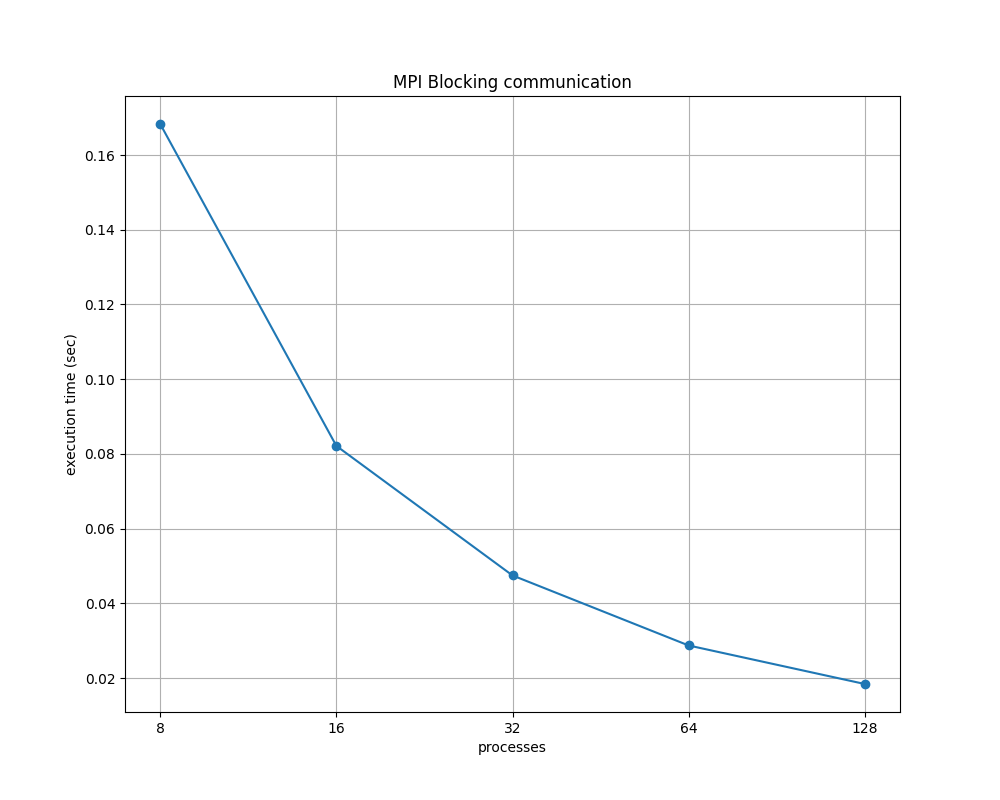
\includegraphics[width=0.8\textwidth]{graph-pi-blocking.png}
        \caption{MPI Blocking Communication between 8 to 128 processes}
        \label{fig:blocking}
    \end{figure}
% deepikat@beskow-login2:/cfs/klemming/scratch/d/deepikat/pi> srun -n 5 ./pi_blocking.out 
% pi: 3.141475
% Execution Time: 0.181464
% deepikat@beskow-login2:/cfs/klemming/scratch/d/deepikat/pi> srun -n 8 ./pi_blocking.out 
% pi: 3.141570
% Execution Time: 0.168313
% deepikat@beskow-login2:/cfs/klemming/scratch/d/deepikat/pi> srun -n 16 ./pi_blocking.out 
% pi: 3.141408
% Execution Time: 0.082145
% deepikat@beskow-login2:/cfs/klemming/scratch/d/deepikat/pi> srun -n 32 ./pi_blocking.out 
% pi: 3.141634
% Execution Time: 0.047470
% deepikat@beskow-login2:/cfs/klemming/scratch/d/deepikat/pi> srun -n 64 ./pi_blocking.out 
% pi: 3.141428
% Execution Time: 0.028720
% deepikat@beskow-login2:/cfs/klemming/scratch/d/deepikat/pi> srun -n 128 ./pi_blocking.out 
% pi: 3.141850
% Execution Time: 0.018408


    \item Answer the following questions:
    \begin{itemize}
        \item Why are \texttt{MPI\_Send()} and \texttt{MPI\_Recv()} called "blocking" communication?\\
         \texttt{MPI\_Send()} and \texttt{MPI\_Recv()} do not return before the MPI buffer is safe for reuse, i.e., they "block" further execution of the program till communication completes.
        \item What is the MPI function for timing?\\
        \texttt{MPI\_Wtime()} enables the measurement of wall time with MPI.
    \end{itemize}
\end{enumerate}

\subsection{MPI Blocking Communication \& Binary Tree Reduction Communication Algorithm}

\end{document}

